%
% Copyright (c) 1996 Bunyip Information Systems Inc.
% All rights reserved
%
% Archie 3.5
% August 1996
%
% overview.tex
%




\chapter{System Overview}
\label{chap:overview}

In order to be able to configure the Archie system properly for your site, you
will need a thorough understanding of the Archie system architecture. This
section introduces more Archie system concepts, to prepare you for the
configuration instructions (in ``Configuring the Basic System'' on
page~\pageref{chap:configure}). First, a whirlwind tour of Archie.

\section{An Archie-eye view}


On first inspection, the Archie system can appear overwhelmingly complex. In
fact, Archie is a straightforward tool for resource discovery in the Internet
environment. Its apparent complexity stems from the fact that it both seeks
out and provides information to Internet users, and it maintains information
on several levels. The following scenario is designed to help de-mystify some
of the operation of the Archie system.
Consider the sample Internet subset in the diagram below:

\begin{figure}[!h]
\begin{center}
\epsfig{file=figs/overview.eps,height=2in}
\end{center}
\caption{Basic Archie Relationships}
\end{figure}

%
%
%
\subsection{Archie as an information accessor}

Suppose AnArchieServer is configured so that it maintains information about
the contents of the anonymous FTP archives at PurpleDataHost and at
BrownDataHost. This means that AnArchieServer has an anonftp
catalog. Furthermore, suppose AnArchieServer keeps a catalog to track the
tech papers available on the Internet (only available at PurpleDataHost, in
this scenario).

To support its operation, AnArchieServer maintains Data Host Information Files
to store information about the particularities of PurpleDataHost and
BrownDataHost. The catalog contains information about each data host's
Internet address, operating system type, available information (technical
papers and/or anonymous ftp archives), etc. This is described more fully
below.

Periodically, AnArchieServer will access the data hosts it knows about (i.e.,
PurpleDataHost and BrownDataHost, here) and determine if the available
information (anonymous FTP files, tech papers) have changed. If so, the anonftp
and tech papers catalogs at AnArchieServer are updated to reflect the changes.

%
%
%
\subsection{Archie as an information provider}

Once AnArchieServer has been set up as described above, people looking for
information (either technical papers or anonymous FTP files) can query various
programs running on AnArchieServer directly. For instance, an individual user
can formulate a query of AnArchieServer's tech papers catalog to determine
which technical papers are of interest. The AnArchieServer tech papers catalog
would be able to supply the Internet address of PurpleDataHost, as well as the
location of the particular technical papers in PurpleDataHost's
repository. Similarly, if a user was looking for information available by
Anonymous FTP, consultation of AnArchieServer's anonftp catalog would allow
the user to select which files to get, from which anonymous ftp archive,
before actually accessing either of PurpleDataHost or BrownDataHost. In fact,
the user need not know, in advance, what Internet sites are data hosts, or
which data hosts provide information: AnArchieServer provides this information
as it is needed.





%
%
%

\section{The two faces of the Archie system}

The Archie system is an information mediator in the sense that it both seeks
out information from other sites on the Internet and provides users access to
the resulting catalogs.


\begin{figure}[!htb]
\begin{center}
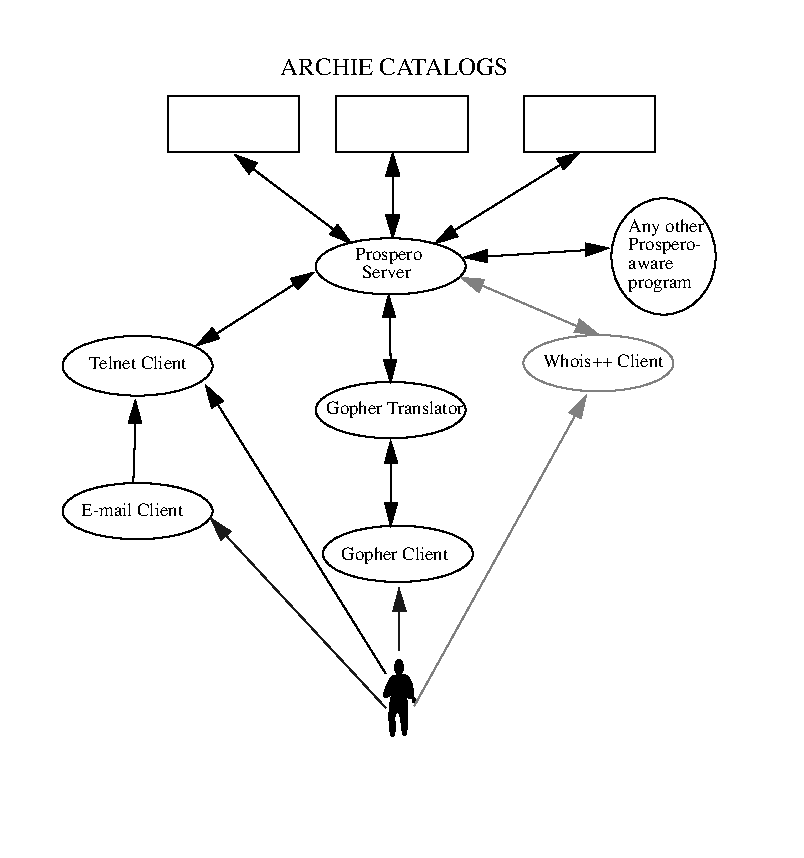
\epsfig{file=figs/catalogs.eps,height=4in}
\end{center}
\caption{User access to the Archie catalogs}
\label{fig:catalogs}
\end{figure}

The information provider aspect of the Archie system is shown in Figure~\ref{fig:catalogs}.
Originally, the Archie system used a modified Prospero File System server
({\bf dirsrv}) to provide user access to its catalogs.  Another module
has been added to the system to access the catalogs via WWW
browsers. \new


The Archie system catalogs are maintained by the Update Cycle processes shown
and described in the following pages. This is illustrated in Figure~\ref{fig:cycle}.


\begin{figure}[!htb]
\begin{center}
\epsfig{file=figs/cycle.eps}
\end{center}
\caption{The Archie update cyle}
\label{fig:cycle}
\end{figure}

Of more immediate importance to Archie system administrators is the
information-seeker aspect of the Archie system. This is composed of several
components which work together to retrieve, parse and update data in the
Archie databases, and is illustrated in Figure~\ref{fig:process}.


\section{Overview of the Archie Update Cycle}

First, some useful definitions:

\begin{itemize}

\item
The catalogs are the collection files which are consulted when a user
carries out an Archie search. For example, the anonftp catalog contains an
index of the files available from anonymous FTP archives on the Internet while
the webindex catalog indexes the WWW space.

\item
The term Data Hosts refers to those network sites which contain the
information that the Archie system will hold in its catalogs.

\item
The Host Information Files or Host Databases contain the latest information
about each of the Data Hosts and the data stored there. The Host Information
File Manager is responsible for maintaining these files.

\item
From the perspective of the Archie administrator, Archie servers fall into
two categories. The local Archie host (site, server) is the one that the
administrator is responsible for maintaining. Remote Archie hosts (sites,
servers) are all those other sites on which the Archie system is being run.

\item
Each component is controlled by a component manager.

\end{itemize}



The major steps of the Update Cycle are:


\begin{itemize}

\item
The Retrieval Component consults the Host Information Files to determine
which Data Hosts should be scheduled for inspection. This information is used
to start the Update Cycle; the rest of the Cycle is
concerned with accessing these sites and retrieving any new data.

\item
The Data Acquisition component is concerned with obtaining any new data
directly from the Data Hosts for which the Archie server is responsible.

\item
The Parse Component is responsible for parsing the incoming data into a form
suitable for the update of the Archie server's catalogs. This often means
removing extraneous information (filtering), as well as performing data
conversions, collation and compression.

\item
The Exchange Component obtains data from remote Archie
servers, if it has been configured to do so. Data so obtained is inserted into
an appropriate place in the Update Cycle and is ultimately incorporated into
the Archie catalogs on the local Archie host.

\item
 Finally, the Update Component obtains the parsed data and integrates it into
the appropriate Archie catalog files. This entails updating the catalogs with
the information obtained from the Data Hosts (or other Archie servers), as
well as making changes to the Host Information Files. Recall that the Host
Information Files contain information such as the last time a Data Host was
accessed for inspection; this information must be brought up to date at the
end of each Update Cycle.

\end{itemize}


Before describing the Update Cycle process in more detail, some important
concepts need to be described.

In order to carry out its processing, the Archie system must maintain special
information about the Data Hosts from which it gets information, and the
status of the information stored in the Archie catalogs that has been obtained
from those sites. These particulars are stored in files collectively referred
to as the Host Information Files. They are maintained by the host\_manage
program.

The Host Information Files fall into two categories: a primary information
file and (possibly) several auxiliary information files. These reside in


\path{\archie/db/host\_db/host-db.dir}

and

\path{\archie/db/host\_db/host-db.pag}


The primary host information file contains particulars about the physical Data
Host itself:


\begin{itemize}
\item the primary name of a site

\item the primary IP address

\item the operating system (if known)

\item timezone (if known)

\item access methods (catalog names)

\end{itemize}


\begin{figure}[!htb]
\begin{center}
\epsfig{file=figs/process.eps,height=6in}
\end{center}
\caption{The Archie system process interactions}
\label{fig:process}
\end{figure}


The Archie server also maintains auxiliary Host Information Files in


\path{\archie/db/host\_db/hostaux-db.dir}

and

\path{\archie/db/host\_db/hostaux-db.pag}


These contain details for a particular Archie catalog. For example, if the
Archie server is keeping track of the anonymous FTP listings of the site
bunyip.com, there would be an entry in the auxiliary files for
bunyip.com/anonftp.

These files contain, in part:

\begin{itemize}
\item The name of the Archie catalog (e.g., anonftp or webindex)

\item The preferred name (that is Domain Name System CNAME, if set)

\item Source Archie server

\item Time of last data retrieval

\item Time of last data parse

\item Time of last update

\item Number of records (catalog-specific definition)

\item Number of times an update has failed

\item  Any comment that the Archie system has seen fit to communicate to the
administrator (reasons for failure of update for example)

\item The current status of the information service at the Data Host (active,
inactive etc.)

\item The name of the Archie host responsible for monitoring this site (for
those cases in which the data is being exchanged between Archie hosts)
\end{itemize}

The Data Host Information Files are maintained by the host\_manage program,
which is described in ``Managing the Host Information Files'' on
page~\pageref{chap:hostmanage}.

Every piece of New Data introduced in the Archie Update Cycle begins with an
Archie header record. This contains all the information necessary for the
various components to process the data obtained from the Data Host. The
information in the header is modified throughout the Cycle to reflect the
changing status of the data. Much of the final information in the header
record is used to update the Host Information Files at the end of the
Cycle. While in most cases the Archie system administrator need not be
concerned with the header records of data within the Archie system, it is
useful to know what the record contains, if problems should occur.

In some cases, the header itself contains all the data necessary to complete
the Update Cycle. For example, for an Archie catalog describing the status
(reachable or unreachable) of sites on a network, an indication of ``success''
or ``failure'' in the header would be enough to know whether to proceed with the
update.

The header is in printable ASCII characters and is human-readable regardless
of the format of other data which may follow it. All headers start with
the string @header\_begin and are terminated with @header\_end. The data itself
starts immediately after the final NEWLINE of the termination string.

\alertbox{It is not advisable to edit Archie data files, especially if the
data is in binary form. Most text editors do not correctly handle binary
files.}

A description of the header can be found in Appendix~\ref{app:header}.
Currently, all header fields are optional, with the exception of the primary
hostname entry.

\section{Update Cycle file naming conventions}

All data files created and maintained during the Update Cycle have the
following naming convention:

\texttt{<primary site name>-<dbname>[\_<id number>].<phase suffix>[<temp>]}

\noindent where

\begin{TTentry}{<primary site name>}

\item[<primary site name>]
is the name of the Data Host.

\item[<dbname>]
is the name of the Archie catalog to be updated with this data.

\item[<id number>]
is an arbitrary number determined by components of the Update
cycle to prevent name clashes (i.e. when there is more that one set of data
associated with the \Param{<primary site name>/<dbname>} pair). Note that this is
OPTIONAL and may not occur in certain file names.

\item[<phase suffix>]
is one of retr, parse or update specifying which part of the
update cycle the data is destined for, not from which the data came.

\item[<temp>]
is a string appended to the name if the current file has a temporary
status, i.e. is undergoing a data transformation (such as being
uncompressed). Currently this is ``\_t''.

\end{TTentry}

\noindent An example using this naming scheme is:

\path{bunyip.com-anonftp\_54.parse\_t}


\alertbox{All files undergoing processing are stored in the \archie/db/tmp
(``holding'') directory, unless otherwise specified (using the ``-t'' switch).}


\alertbox{The manual pages describe how to override the default holding
directory for the Archie programs. However, the directory you choose instead
of \Path{\archie/db/tmp} must not be on a different filesystem (partition) from
\archie, as the programs make use of ``hard links'' which cannot cross partition
boundaries. See ln(1).}



%
%
%
\section{Process naming conventions}

By reading the header record the controlling process of Archie's Update Cycle
automatically generates the name of the appropriate program to invoke for the
successive phases in data processing. The syntax for the process name is

\path{<component name>\_<dbname>[\_<os type>]}

\noindent where

\begin{TTentry}{<component name>}
\item[<component name>] is one of retrieve, parse, update or net

\item[<dbame>]
is the name of the Archie catalog with which this data is associated

\item[<os type>]
is optional and is used when different operating systems require
different processing functions (e.g., when parsing a UNIX, Novell or
VMS anonymous FTP listing).
\end{TTentry}


For example, if the control program reads a header which specifies that this
data is destined for an anonymous FTP catalog, and that it requires parsing,
the control program will invoke the parse\_anonftp program. This program may,
in turn, look at the header and determine that it is a UNIX BSD listing and
will invoke parse\_anonftp\_unix\_bsd on the data file for processing.


\alertbox{There will be cases in which the operation to be performed is
similar enough that the same program may be used for more than one purpose. In
this case soft links, which follow the naming convention, are made
to a single program.}

The update process is complex and requires consistent and complete information
in order to complete successfully. This means it is possible to have a failure
at any step in the Update Cycle. For example, the data host may not be
reachable, or the parsing of the obtained data may fail. In this case, the
program will produce a file containing a header reflecting the nature of the
failure. This usually contains an explanation of how or why the failure
occurred (this is signified in the header record by the comment field). The
``failed'' data continues to be passed through the Update Cycle and at each
phase the header is updated to reflect what has happened to it. Thus, even
though the data acquisition has failed, the last\_parsed field of the header
will be updated.


%
%
%

\section{The Update Cycle in detail}
\label{sec:update}
Now, each component of the Update Cycle will be discussed in some detail.

The Update Cycle is performed, step by step, under the guidance of the
arcontrol program. It is invoked in different modes depending on the phase of
the Cycle desired. It scans the holding directory for the appropriate data
files and may perform some basic data transformations on those files (such as
uncompressing the data) before passing them on to the appropriate programs for
processing.

The steps followed by the system are as follows:


\subsection{The Retrieval Component (arretrieve)}

This component is responsible for querying the local Archie system for the
list of sites scheduled for inspection. It does so by contacting the local
Archie arserver process (see ``The arserver program'' on page 34) and
downloading a set of headers corresponding to those Data Host/catalog
combinations. Each header is placed in a separate file, ready for the Data
Acquisition phase of the cycle.

\subsection{The Data Acquisition Component (arcontrol -r)}

arcontrol examines the header files (created by the Retrieval Component). For
each Data Host/catalog pair, it determines the appropriate process for
retrieving new data for the catalog from the Data Host. arcontrol invokes the
selected process, passing the name of the header file as a parameter. Once the
process has finished acquiring information from the Data Host, a file
containing the results will be created (according to the scheme outlined in
``Update Cycle file naming conventions'' on page 23). The file will contain the
header record and either retrieved data or an indication of failure.

\subsection{The Parse Component (arcontrol -p)}

Managed by arcontrol, the processes responsible will parse the files generated
by the Data Acquisition Component into the appropriate form for the target
catalog. For example, in the case of anonymous FTP listings, it will take the
raw data and create an output file of the correct form for insertion into the
anonftp catalog.

\subsection{The Update Component (arcontrol -u)}

Invoked by arcontrol, the Update Component process performs two functions: it
will update the Host Information Files, and it will update the Archie catalog
itself. For example, when a correctly parsed anonftp (anonymous FTP) listing
from bunyip.com is ready, the data itself is inserted into the anonftp catalog
and the record for ``bunyip.com.anonftp'' is modified in the auxiliary Host
Information Files.


\section{Data Exchange}

This release of Archie allows the exchange of arbitrary catalog data between
cooperating Archie systems. A basic flooding i-have/send-me algorithm, similar
to that used in the Internet USENET news system, is used to maintain weak
consistency between an arbitrary number of Archie servers. ``Virtual'' networks
of Archie systems can be created and any individual server may belong to zero
or more of these data-exchange networks.

This allows a multi-tiered system (such as the example on the map) whereby
certain key sites may be responsible for inter-continental data exchanges and
others would feed from them, instead of every Archie site having to contact
all others worldwide.




\section{Conclusion}

This concludes the description of the Archie Update Cycle processes. With a
better understanding of how Archie works, you should be now be ready to
configure your Archie server to fulfill your needs. The discussion of Archie
configuration begins in section~\ref{chap:configure}, ``Configuring the Basic System'' .


